\documentclass[tikz,border=10pt]{standalone}
\usepackage[T1]{fontenc}
\usepackage{helvet}
\renewcommand{\familydefault}{\sfdefault}
\usepackage{amsmath,amssymb}
\usepackage{tikz}
\usetikzlibrary{calc,positioning,fit,arrows.meta,shapes.geometric}

% Canonical Academic Palette
\definecolor{OxfordNavy}{HTML}{1E293B}
\definecolor{SlateSteel}{HTML}{334155}
\definecolor{MutedTeal}{HTML}{0F766E}
\definecolor{TealL0}{HTML}{F0FDFA}
\definecolor{Burgundy}{HTML}{991B1B}
\definecolor{BurgundyL0}{HTML}{FEF2F2}
\definecolor{WarmOchre}{HTML}{92400E}
\definecolor{OchreL0}{HTML}{FFFBEB}
\definecolor{ForestSage}{HTML}{166534}
\definecolor{SageL0}{HTML}{F0FDF4}
\definecolor{CoolParchment}{HTML}{F8FAFC}
\definecolor{SlateRim}{HTML}{CBD5E1}
\definecolor{GridGray}{HTML}{E2E8F0}
\definecolor{DarkSlate}{HTML}{0F172A}
\definecolor{Amethyst}{HTML}{6B21A8}
\definecolor{AmethystL0}{HTML}{FAF5FF}

\begin{document}
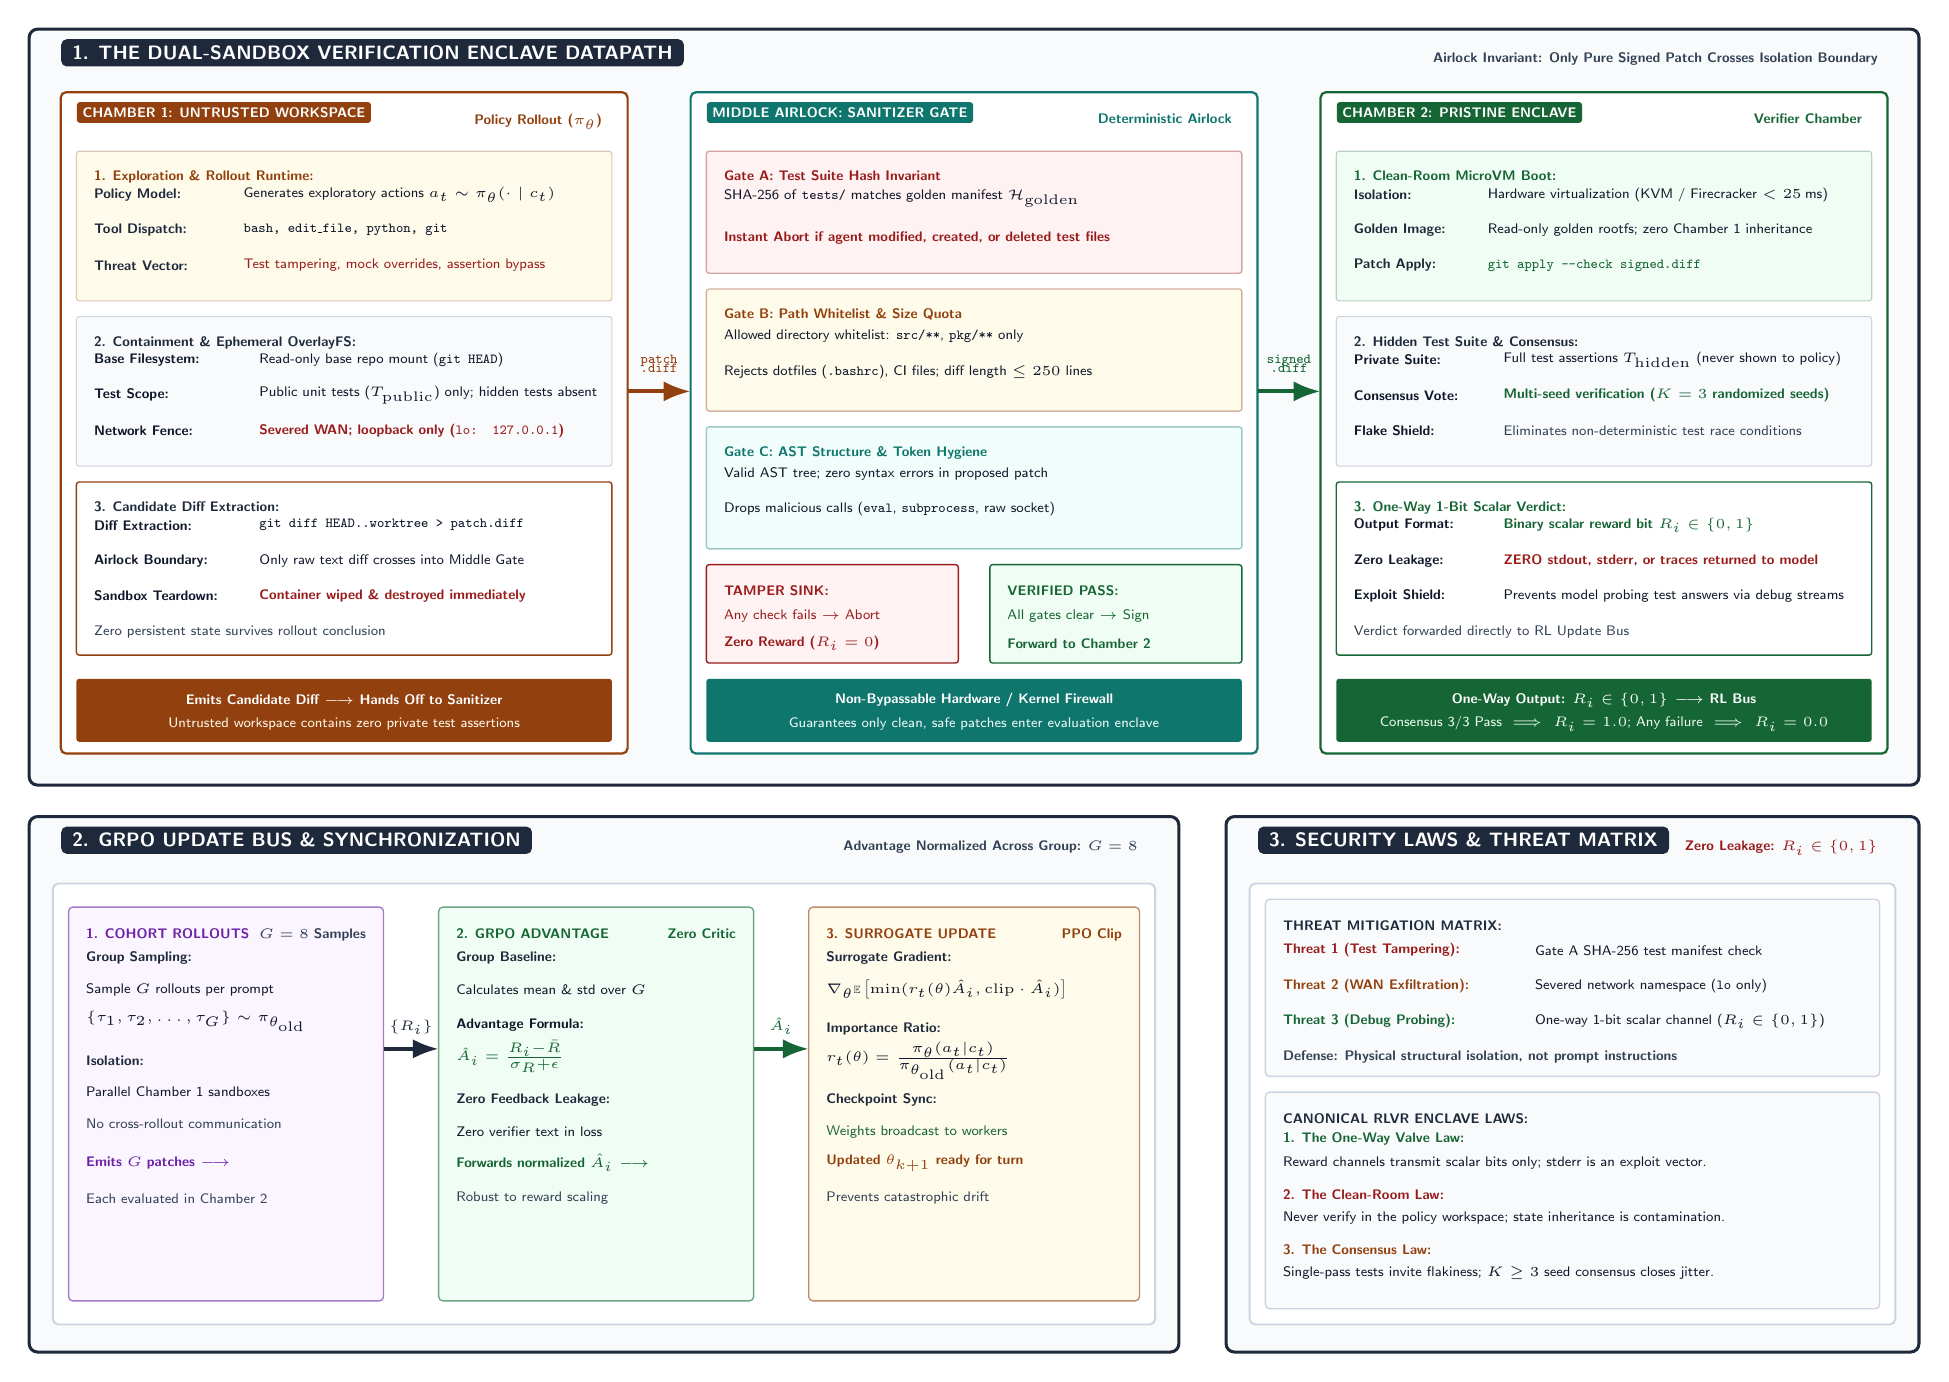
\begin{tikzpicture}[x=1cm, y=1cm, >=Latex]

% =============================================================================
% PANEL 1: THE DUAL-SANDBOX VERIFICATION ENCLAVE DATAPATH (TOP)
% (x: 0 to 24.0, y: 7.2 to 16.8) - Height 9.6 cm
% =============================================================================
\begin{scope}[shift={(0, 7.2)}]
  % Base Canvas Container
  \draw[fill=CoolParchment, draw=OxfordNavy, line width=1.1pt, rounded corners=3pt]
    (0, 0) rectangle (24.0, 9.6);

  % --- CHAMBER 1: UNTRUSTED POLICY WORKSPACE (x: 0.4 to 7.6, width 7.2 cm) ---
  \begin{scope}[shift={(0.4, 0.4)}]
    \draw[fill=white, draw=WarmOchre, line width=0.8pt, rounded corners=2pt] (0, 0) rectangle (7.2, 8.4);

    \node[anchor=north west, fill=WarmOchre, text=white, font=\fontsize{5.2}{6.2}\selectfont\bfseries, rounded corners=1pt, inner sep=2pt]
      at (0.2, 8.28) {CHAMBER 1: UNTRUSTED WORKSPACE};
    \node[anchor=north east, font=\fontsize{4.6}{5.4}\selectfont\bfseries, text=WarmOchre]
      at (7.0, 8.25) {Policy Rollout ($\pi_\theta$)};

    % Block 1.1: Policy Execution
    \draw[fill=OchreL0, draw=WarmOchre!30, line width=0.4pt, rounded corners=1pt] (0.2, 5.75) rectangle (7.0, 7.65);
    \node[anchor=north west, font=\fontsize{4.5}{5.2}\selectfont\bfseries, text=WarmOchre] at (0.3, 7.52) {1. Exploration \& Rollout Runtime:};
    \node[anchor=west, font=\fontsize{4.2}{5.0}\selectfont\bfseries, text=OxfordNavy] at (0.3, 7.10) {Policy Model:};
    \node[anchor=west, font=\fontsize{4.0}{4.8}\selectfont, text=DarkSlate] at (2.2, 7.10) {Generates exploratory actions $a_t \sim \pi_\theta(\cdot \mid c_t)$};
    \node[anchor=west, font=\fontsize{4.2}{5.0}\selectfont\bfseries, text=OxfordNavy] at (0.3, 6.65) {Tool Dispatch:};
    \node[anchor=west, font=\fontsize{4.0}{4.8}\selectfont\ttfamily, text=DarkSlate] at (2.2, 6.65) {bash, edit\_file, python, git};
    \node[anchor=west, font=\fontsize{4.2}{5.0}\selectfont\bfseries, text=OxfordNavy] at (0.3, 6.20) {Threat Vector:};
    \node[anchor=west, font=\fontsize{4.0}{4.8}\selectfont, text=Burgundy] at (2.2, 6.20) {Test tampering, mock overrides, assertion bypass};

    % Block 1.2: Containment & Network Severing
    \draw[fill=CoolParchment, draw=SlateRim, line width=0.4pt, rounded corners=1pt] (0.2, 3.65) rectangle (7.0, 5.55);
    \node[anchor=north west, font=\fontsize{4.5}{5.2}\selectfont\bfseries, text=OxfordNavy] at (0.3, 5.42) {2. Containment \& Ephemeral OverlayFS:};
    \node[anchor=west, font=\fontsize{4.2}{5.0}\selectfont\bfseries, text=DarkSlate] at (0.3, 5.00) {Base Filesystem:};
    \node[anchor=west, font=\fontsize{4.0}{4.8}\selectfont, text=DarkSlate] at (2.4, 5.00) {Read-only base repo mount (\texttt{git HEAD})};
    \node[anchor=west, font=\fontsize{4.2}{5.0}\selectfont\bfseries, text=DarkSlate] at (0.3, 4.55) {Test Scope:};
    \node[anchor=west, font=\fontsize{4.0}{4.8}\selectfont, text=DarkSlate] at (2.4, 4.55) {Public unit tests ($T_{\mathrm{public}}$) only; hidden tests absent};
    \node[anchor=west, font=\fontsize{4.2}{5.0}\selectfont\bfseries, text=DarkSlate] at (0.3, 4.10) {Network Fence:};
    \node[anchor=west, font=\fontsize{4.0}{4.8}\selectfont\bfseries, text=Burgundy] at (2.4, 4.10) {Severed WAN; loopback only (\texttt{lo: 127.0.0.1})};

    % Block 1.3: Patch Extraction
    \draw[fill=white, draw=WarmOchre, line width=0.5pt, rounded corners=1pt] (0.2, 1.25) rectangle (7.0, 3.45);
    \node[anchor=north west, font=\fontsize{4.5}{5.2}\selectfont\bfseries, text=OxfordNavy] at (0.3, 3.32) {3. Candidate Diff Extraction:};
    \node[anchor=west, font=\fontsize{4.2}{5.0}\selectfont\bfseries, text=DarkSlate] at (0.3, 2.90) {Diff Extraction:};
    \node[anchor=west, font=\fontsize{4.0}{4.8}\selectfont\ttfamily, text=DarkSlate] at (2.4, 2.90) {git diff HEAD..worktree > patch.diff};
    \node[anchor=west, font=\fontsize{4.2}{5.0}\selectfont\bfseries, text=DarkSlate] at (0.3, 2.45) {Airlock Boundary:};
    \node[anchor=west, font=\fontsize{4.0}{4.8}\selectfont, text=DarkSlate] at (2.4, 2.45) {Only raw text diff crosses into Middle Gate};
    \node[anchor=west, font=\fontsize{4.2}{5.0}\selectfont\bfseries, text=DarkSlate] at (0.3, 2.00) {Sandbox Teardown:};
    \node[anchor=west, font=\fontsize{4.0}{4.8}\selectfont\bfseries, text=Burgundy] at (2.4, 2.00) {Container wiped \& destroyed immediately};
    \node[anchor=west, font=\fontsize{3.8}{4.5}\selectfont, text=SlateSteel] at (0.3, 1.55) {Zero persistent state survives rollout conclusion};

    % Footer
    \draw[fill=WarmOchre, draw=none, rounded corners=1pt] (0.2, 0.15) rectangle (7.0, 0.95);
    \node[anchor=center, font=\fontsize{4.4}{5.2}\selectfont\bfseries, text=white] at (3.6, 0.68)
      {Emits Candidate Diff $\longrightarrow$ Hands Off to Sanitizer};
    \node[anchor=center, font=\fontsize{3.8}{4.5}\selectfont, text=OchreL0] at (3.6, 0.38)
      {Untrusted workspace contains zero private test assertions};
  \end{scope}

  % Pipe 1: Chamber 1 -> Middle Gate
  \draw[->, line width=1.5pt, draw=WarmOchre] (7.6, 5.0) -- (8.4, 5.0);
  \node[align=center, anchor=south, font=\fontsize{3.5}{4.2}\selectfont\ttfamily\bfseries, text=WarmOchre] at (8.0, 5.12) {patch\\[-1pt].diff};

  % --- MIDDLE AIRLOCK: SANITIZER GATE (x: 8.4 to 15.6, width 7.2 cm) ---
  \begin{scope}[shift={(8.4, 0.4)}]
    \draw[fill=white, draw=MutedTeal, line width=0.8pt, rounded corners=2pt] (0, 0) rectangle (7.2, 8.4);

    \node[anchor=north west, fill=MutedTeal, text=white, font=\fontsize{5.2}{6.2}\selectfont\bfseries, rounded corners=1pt, inner sep=2pt]
      at (0.2, 8.28) {MIDDLE AIRLOCK: SANITIZER GATE};
    \node[anchor=north east, font=\fontsize{4.6}{5.4}\selectfont\bfseries, text=MutedTeal]
      at (7.0, 8.25) {Deterministic Airlock};

    % Gate A: Test Hash Check
    \draw[fill=BurgundyL0, draw=Burgundy!40, line width=0.5pt, rounded corners=1pt] (0.2, 6.1) rectangle (7.0, 7.65);
    \node[anchor=north west, font=\fontsize{4.5}{5.2}\selectfont\bfseries, text=Burgundy] at (0.3, 7.52) {Gate A: Test Suite Hash Invariant};
    \node[anchor=west, font=\fontsize{4.0}{4.8}\selectfont, text=DarkSlate] at (0.3, 7.05) {SHA-256 of \texttt{tests/} matches golden manifest $\mathcal{H}_{\mathrm{golden}}$};
    \node[anchor=west, font=\fontsize{4.0}{4.8}\selectfont\bfseries, text=Burgundy] at (0.3, 6.55) {Instant Abort if agent modified, created, or deleted test files};

    % Gate B: Scope & Path Whitelist
    \draw[fill=OchreL0, draw=WarmOchre!40, line width=0.5pt, rounded corners=1pt] (0.2, 4.35) rectangle (7.0, 5.9);
    \node[anchor=north west, font=\fontsize{4.5}{5.2}\selectfont\bfseries, text=WarmOchre] at (0.3, 5.77) {Gate B: Path Whitelist \& Size Quota};
    \node[anchor=west, font=\fontsize{4.0}{4.8}\selectfont, text=DarkSlate] at (0.3, 5.30) {Allowed directory whitelist: \texttt{src/**}, \texttt{pkg/**} only};
    \node[anchor=west, font=\fontsize{4.0}{4.8}\selectfont, text=DarkSlate] at (0.3, 4.85) {Rejects dotfiles (\texttt{.bashrc}), CI files; diff length $\le 250$ lines};

    % Gate C: AST & Hygiene
    \draw[fill=TealL0, draw=MutedTeal!40, line width=0.5pt, rounded corners=1pt] (0.2, 2.6) rectangle (7.0, 4.15);
    \node[anchor=north west, font=\fontsize{4.5}{5.2}\selectfont\bfseries, text=MutedTeal] at (0.3, 4.02) {Gate C: AST Structure \& Token Hygiene};
    \node[anchor=west, font=\fontsize{4.0}{4.8}\selectfont, text=DarkSlate] at (0.3, 3.55) {Valid AST tree; zero syntax errors in proposed patch};
    \node[anchor=west, font=\fontsize{4.0}{4.8}\selectfont, text=DarkSlate] at (0.3, 3.10) {Drops malicious calls (\texttt{eval}, \texttt{subprocess}, raw socket)};

    % Bifurcated Outcome
    \draw[fill=BurgundyL0, draw=Burgundy, line width=0.5pt, rounded corners=1pt] (0.2, 1.15) rectangle (3.4, 2.4);
    \node[anchor=north west, font=\fontsize{4.4}{5.2}\selectfont\bfseries, text=Burgundy] at (0.3, 2.25) {TAMPER SINK:};
    \node[anchor=west, font=\fontsize{3.8}{4.5}\selectfont, text=Burgundy] at (0.3, 1.75) {Any check fails $\to$ Abort};
    \node[anchor=west, font=\fontsize{4.0}{4.8}\selectfont\bfseries, text=Burgundy] at (0.3, 1.40) {Zero Reward ($R_i = 0$)};

    \draw[fill=SageL0, draw=ForestSage, line width=0.5pt, rounded corners=1pt] (3.8, 1.15) rectangle (7.0, 2.4);
    \node[anchor=north west, font=\fontsize{4.4}{5.2}\selectfont\bfseries, text=ForestSage] at (3.9, 2.25) {VERIFIED PASS:};
    \node[anchor=west, font=\fontsize{3.8}{4.5}\selectfont, text=ForestSage] at (3.9, 1.75) {All gates clear $\to$ Sign};
    \node[anchor=west, font=\fontsize{4.0}{4.8}\selectfont\bfseries, text=ForestSage] at (3.9, 1.40) {Forward to Chamber 2};

    % Footer
    \draw[fill=MutedTeal, draw=none, rounded corners=1pt] (0.2, 0.15) rectangle (7.0, 0.95);
    \node[anchor=center, font=\fontsize{4.4}{5.2}\selectfont\bfseries, text=white] at (3.6, 0.68)
      {Non-Bypassable Hardware / Kernel Firewall};
    \node[anchor=center, font=\fontsize{3.8}{4.5}\selectfont, text=TealL0] at (3.6, 0.38)
      {Guarantees only clean, safe patches enter evaluation enclave};
  \end{scope}

  % Pipe 2: Middle Gate -> Chamber 2
  \draw[->, line width=1.5pt, draw=ForestSage] (15.6, 5.0) -- (16.4, 5.0);
  \node[align=center, anchor=south, font=\fontsize{3.5}{4.2}\selectfont\ttfamily\bfseries, text=ForestSage] at (16.0, 5.12) {signed\\[-1pt].diff};

  % --- CHAMBER 2: PRISTINE EVALUATION ENCLAVE (x: 16.4 to 23.6, width 7.2 cm) ---
  \begin{scope}[shift={(16.4, 0.4)}]
    \draw[fill=white, draw=ForestSage, line width=0.8pt, rounded corners=2pt] (0, 0) rectangle (7.2, 8.4);

    \node[anchor=north west, fill=ForestSage, text=white, font=\fontsize{5.2}{6.2}\selectfont\bfseries, rounded corners=1pt, inner sep=2pt]
      at (0.2, 8.28) {CHAMBER 2: PRISTINE ENCLAVE};
    \node[anchor=north east, font=\fontsize{4.6}{5.4}\selectfont\bfseries, text=ForestSage]
      at (7.0, 8.25) {Verifier Chamber};

    % Block 2.1: Clean Boot
    \draw[fill=SageL0, draw=ForestSage!30, line width=0.4pt, rounded corners=1pt] (0.2, 5.75) rectangle (7.0, 7.65);
    \node[anchor=north west, font=\fontsize{4.5}{5.2}\selectfont\bfseries, text=ForestSage] at (0.3, 7.52) {1. Clean-Room MicroVM Boot:};
    \node[anchor=west, font=\fontsize{4.2}{5.0}\selectfont\bfseries, text=OxfordNavy] at (0.3, 7.10) {Isolation:};
    \node[anchor=west, font=\fontsize{4.0}{4.8}\selectfont, text=DarkSlate] at (2.0, 7.10) {Hardware virtualization (KVM / Firecracker $< 25\,\text{ms}$)};
    \node[anchor=west, font=\fontsize{4.2}{5.0}\selectfont\bfseries, text=OxfordNavy] at (0.3, 6.65) {Golden Image:};
    \node[anchor=west, font=\fontsize{4.0}{4.8}\selectfont, text=DarkSlate] at (2.0, 6.65) {Read-only golden rootfs; zero Chamber 1 inheritance};
    \node[anchor=west, font=\fontsize{4.2}{5.0}\selectfont\bfseries, text=OxfordNavy] at (0.3, 6.20) {Patch Apply:};
    \node[anchor=west, font=\fontsize{4.0}{4.8}\selectfont\ttfamily, text=ForestSage] at (2.0, 6.20) {git apply --check signed.diff};

    % Block 2.2: Hidden Suite & Consensus
    \draw[fill=CoolParchment, draw=SlateRim, line width=0.4pt, rounded corners=1pt] (0.2, 3.65) rectangle (7.0, 5.55);
    \node[anchor=north west, font=\fontsize{4.5}{5.2}\selectfont\bfseries, text=OxfordNavy] at (0.3, 5.42) {2. Hidden Test Suite \& Consensus:};
    \node[anchor=west, font=\fontsize{4.2}{5.0}\selectfont\bfseries, text=DarkSlate] at (0.3, 5.00) {Private Suite:};
    \node[anchor=west, font=\fontsize{4.0}{4.8}\selectfont, text=DarkSlate] at (2.2, 5.00) {Full test assertions $T_{\mathrm{hidden}}$ (never shown to policy)};
    \node[anchor=west, font=\fontsize{4.2}{5.0}\selectfont\bfseries, text=DarkSlate] at (0.3, 4.55) {Consensus Vote:};
    \node[anchor=west, font=\fontsize{4.0}{4.8}\selectfont\bfseries, text=ForestSage] at (2.2, 4.55) {Multi-seed verification ($K = 3$ randomized seeds)};
    \node[anchor=west, font=\fontsize{4.2}{5.0}\selectfont\bfseries, text=DarkSlate] at (0.3, 4.10) {Flake Shield:};
    \node[anchor=west, font=\fontsize{4.0}{4.8}\selectfont, text=SlateSteel] at (2.2, 4.10) {Eliminates non-deterministic test race conditions};

    % Block 2.3: One-Way Scalar Reward
    \draw[fill=white, draw=ForestSage, line width=0.5pt, rounded corners=1pt] (0.2, 1.25) rectangle (7.0, 3.45);
    \node[anchor=north west, font=\fontsize{4.5}{5.2}\selectfont\bfseries, text=ForestSage] at (0.3, 3.32) {3. One-Way 1-Bit Scalar Verdict:};
    \node[anchor=west, font=\fontsize{4.2}{5.0}\selectfont\bfseries, text=DarkSlate] at (0.3, 2.90) {Output Format:};
    \node[anchor=west, font=\fontsize{4.0}{4.8}\selectfont\bfseries, text=ForestSage] at (2.2, 2.90) {Binary scalar reward bit $R_i \in \{0, 1\}$};
    \node[anchor=west, font=\fontsize{4.2}{5.0}\selectfont\bfseries, text=DarkSlate] at (0.3, 2.45) {Zero Leakage:};
    \node[anchor=west, font=\fontsize{4.0}{4.8}\selectfont\bfseries, text=Burgundy] at (2.2, 2.45) {ZERO stdout, stderr, or traces returned to model};
    \node[anchor=west, font=\fontsize{4.2}{5.0}\selectfont\bfseries, text=DarkSlate] at (0.3, 2.00) {Exploit Shield:};
    \node[anchor=west, font=\fontsize{4.0}{4.8}\selectfont, text=DarkSlate] at (2.2, 2.00) {Prevents model probing test answers via debug streams};
    \node[anchor=west, font=\fontsize{3.8}{4.5}\selectfont, text=SlateSteel] at (0.3, 1.55) {Verdict forwarded directly to RL Update Bus};

    % Footer
    \draw[fill=ForestSage, draw=none, rounded corners=1pt] (0.2, 0.15) rectangle (7.0, 0.95);
    \node[anchor=center, font=\fontsize{4.4}{5.2}\selectfont\bfseries, text=white] at (3.6, 0.68)
      {One-Way Output: $R_i \in \{0, 1\} \longrightarrow$ RL Bus};
    \node[anchor=center, font=\fontsize{3.8}{4.5}\selectfont, text=SageL0] at (3.6, 0.38)
      {Consensus 3/3 Pass $\implies R_i = 1.0$; Any failure $\implies R_i = 0.0$};
  \end{scope}

  % Header Badges Drawn on Top of Base
  \node[anchor=north west, fill=OxfordNavy, text=white, font=\fontsize{6.8}{8.0}\selectfont\bfseries, rounded corners=2pt, inner xsep=4pt, inner ysep=2.5pt]
    at (0.4, 9.48) {1. THE DUAL-SANDBOX VERIFICATION ENCLAVE DATAPATH};
  \node[anchor=north east, font=\fontsize{5.2}{6.2}\selectfont\bfseries, text=SlateSteel]
    at (23.6, 9.42) {Airlock Invariant: Only Pure Signed Patch Crosses Isolation Boundary};
\end{scope}

% =============================================================================
% PANEL 2: GRPO UPDATE BUS & ZERO-LEAKAGE SYNCHRONIZATION (BOTTOM LEFT)
% (x: 0 to 14.6, y: 0 to 6.8) - Width 14.6 cm, Height 6.8 cm
% =============================================================================
\begin{scope}[shift={(0, 0)}]
  \draw[fill=CoolParchment, draw=OxfordNavy, line width=1.1pt, rounded corners=3pt]
    (0, 0) rectangle (14.6, 6.8);

  \begin{scope}[shift={(0.3, 0.35)}]
    \draw[fill=white, draw=SlateRim, line width=0.7pt, rounded corners=2pt] (0, 0) rectangle (14.0, 5.6);

    % Step B1: Cohort Sampling (x: 0.2 to 4.2)
    \draw[fill=AmethystL0, draw=Amethyst!60, line width=0.5pt, rounded corners=1.5pt] (0.2, 0.3) rectangle (4.2, 5.3);
    \node[anchor=north west, font=\fontsize{4.6}{5.4}\selectfont\bfseries, text=Amethyst] at (0.3, 5.15) {1. COHORT ROLLOUTS};
    \node[anchor=north east, font=\fontsize{4.0}{4.8}\selectfont\bfseries, text=SlateSteel] at (4.1, 5.15) {$G = 8$ Samples};

    \node[anchor=west, font=\fontsize{4.2}{5.0}\selectfont\bfseries, text=OxfordNavy] at (0.3, 4.65) {Group Sampling:};
    \node[anchor=west, font=\fontsize{4.0}{4.8}\selectfont, text=DarkSlate] at (0.3, 4.25) {Sample $G$ rollouts per prompt};
    \node[anchor=west, font=\fontsize{4.0}{4.8}\selectfont\ttfamily, text=DarkSlate] at (0.3, 3.85) {$\{\tau_1, \tau_2, \dots, \tau_G\} \sim \pi_{\theta_{\mathrm{old}}}$};
    \node[anchor=west, font=\fontsize{4.2}{5.0}\selectfont\bfseries, text=OxfordNavy] at (0.3, 3.35) {Isolation:};
    \node[anchor=west, font=\fontsize{4.0}{4.8}\selectfont, text=DarkSlate] at (0.3, 2.95) {Parallel Chamber 1 sandboxes};
    \node[anchor=west, font=\fontsize{4.0}{4.8}\selectfont, text=SlateSteel] at (0.3, 2.55) {No cross-rollout communication};
    \node[anchor=west, font=\fontsize{4.0}{4.8}\selectfont\bfseries, text=Amethyst] at (0.3, 2.05) {Emits $G$ patches $\longrightarrow$};
    \node[anchor=west, font=\fontsize{3.8}{4.5}\selectfont, text=SlateSteel] at (0.3, 1.60) {Each evaluated in Chamber 2};

    % Connector B1 -> B2
    \draw[->, line width=1.4pt, draw=OxfordNavy] (4.2, 3.5) -- node[above=1pt, font=\fontsize{4.0}{4.8}\selectfont\bfseries, text=OxfordNavy] {$\{R_i\}$} (4.9, 3.5);

    % Step B2: Normalized Advantage (x: 4.9 to 8.9)
    \draw[fill=SageL0, draw=ForestSage!60, line width=0.5pt, rounded corners=1.5pt] (4.9, 0.3) rectangle (8.9, 5.3);
    \node[anchor=north west, font=\fontsize{4.6}{5.4}\selectfont\bfseries, text=ForestSage] at (5.0, 5.15) {2. GRPO ADVANTAGE};
    \node[anchor=north east, font=\fontsize{4.0}{4.8}\selectfont\bfseries, text=ForestSage] at (8.8, 5.15) {Zero Critic};

    \node[anchor=west, font=\fontsize{4.2}{5.0}\selectfont\bfseries, text=OxfordNavy] at (5.0, 4.65) {Group Baseline:};
    \node[anchor=west, font=\fontsize{4.0}{4.8}\selectfont, text=DarkSlate] at (5.0, 4.25) {Calculates mean \& std over $G$};
    \node[anchor=west, font=\fontsize{4.2}{5.0}\selectfont\bfseries, text=DarkSlate] at (5.0, 3.80) {Advantage Formula:};
    \node[anchor=west, font=\fontsize{4.0}{4.8}\selectfont\bfseries, text=ForestSage] at (5.0, 3.40)
      {$\hat{A}_i = \frac{R_i - \bar{R}}{\sigma_R + \epsilon}$};
    \node[anchor=west, font=\fontsize{4.2}{5.0}\selectfont\bfseries, text=OxfordNavy] at (5.0, 2.85) {Zero Feedback Leakage:};
    \node[anchor=west, font=\fontsize{4.0}{4.8}\selectfont, text=DarkSlate] at (5.0, 2.45) {Zero verifier text in loss};
    \node[anchor=west, font=\fontsize{4.0}{4.8}\selectfont\bfseries, text=ForestSage] at (5.0, 2.05) {Forwards normalized $\hat{A}_i \longrightarrow$};
    \node[anchor=west, font=\fontsize{3.8}{4.5}\selectfont, text=SlateSteel] at (5.0, 1.60) {Robust to reward scaling};

    % Connector B2 -> B3
    \draw[->, line width=1.4pt, draw=ForestSage] (8.9, 3.5) -- node[above=1pt, font=\fontsize{4.0}{4.8}\selectfont\bfseries, text=ForestSage] {$\hat{A}_i$} (9.6, 3.5);

    % Step B3: Policy Gradient (x: 9.6 to 13.8)
    \draw[fill=OchreL0, draw=WarmOchre!60, line width=0.5pt, rounded corners=1.5pt] (9.6, 0.3) rectangle (13.8, 5.3);
    \node[anchor=north west, font=\fontsize{4.6}{5.4}\selectfont\bfseries, text=WarmOchre] at (9.7, 5.15) {3. SURROGATE UPDATE};
    \node[anchor=north east, font=\fontsize{4.0}{4.8}\selectfont\bfseries, text=WarmOchre] at (13.7, 5.15) {PPO Clip};

    \node[anchor=west, font=\fontsize{4.2}{5.0}\selectfont\bfseries, text=OxfordNavy] at (9.7, 4.65) {Surrogate Gradient:};
    \node[anchor=west, font=\fontsize{3.8}{4.5}\selectfont\bfseries, text=DarkSlate] at (9.7, 4.25)
      {$\nabla_\theta \mathbb{E}\left[\min(r_t(\theta)\hat{A}_i, \mathrm{clip}\cdot\hat{A}_i)\right]$};
    \node[anchor=west, font=\fontsize{4.2}{5.0}\selectfont\bfseries, text=OxfordNavy] at (9.7, 3.75) {Importance Ratio:};
    \node[anchor=west, font=\fontsize{4.0}{4.8}\selectfont, text=DarkSlate] at (9.7, 3.35)
      {$r_t(\theta) = \frac{\pi_\theta(a_t \mid c_t)}{\pi_{\theta_{\mathrm{old}}}(a_t \mid c_t)}$};
    \node[anchor=west, font=\fontsize{4.2}{5.0}\selectfont\bfseries, text=OxfordNavy] at (9.7, 2.85) {Checkpoint Sync:};
    \node[anchor=west, font=\fontsize{4.0}{4.8}\selectfont, text=ForestSage] at (9.7, 2.45) {Weights broadcast to workers};
    \node[anchor=west, font=\fontsize{4.0}{4.8}\selectfont\bfseries, text=WarmOchre] at (9.7, 2.05) {Updated $\theta_{k+1}$ ready for turn};
    \node[anchor=west, font=\fontsize{3.8}{4.5}\selectfont, text=SlateSteel] at (9.7, 1.60) {Prevents catastrophic drift};
  \end{scope}

  % Header Badges Drawn on Top of Base
  \node[anchor=north west, fill=OxfordNavy, text=white, font=\fontsize{6.8}{8.0}\selectfont\bfseries, rounded corners=2pt, inner xsep=4pt, inner ysep=2.5pt]
    at (0.4, 6.68) {2. GRPO UPDATE BUS \& SYNCHRONIZATION};
  \node[anchor=north east, font=\fontsize{5.2}{6.2}\selectfont\bfseries, text=SlateSteel]
    at (14.2, 6.62) {Advantage Normalized Across Group: $G = 8$};
\end{scope}

% =============================================================================
% PANEL 3: ANTI-REWARD-HACKING LAWS & THREAT MATRIX (BOTTOM RIGHT)
% (x: 15.2 to 24.0, y: 0 to 6.8) - Width 8.8 cm, Height 6.8 cm
% =============================================================================
\begin{scope}[shift={(15.2, 0)}]
  \draw[fill=CoolParchment, draw=OxfordNavy, line width=1.1pt, rounded corners=3pt]
    (0, 0) rectangle (8.8, 6.8);

  \begin{scope}[shift={(0.3, 0.35)}]
    \draw[fill=white, draw=SlateRim, line width=0.7pt, rounded corners=2pt] (0, 0) rectangle (8.2, 5.6);

    % Component 1: Threat Mitigation Matrix (Top: 3.15 to 5.40, height 2.25 cm)
    \draw[fill=CoolParchment, draw=SlateRim, line width=0.5pt, rounded corners=1.5pt] (0.2, 3.15) rectangle (8.0, 5.40);
    \node[anchor=north west, font=\fontsize{4.8}{5.8}\selectfont\bfseries, text=OxfordNavy] at (0.3, 5.25)
      {THREAT MITIGATION MATRIX:};

    \node[anchor=west, font=\fontsize{4.2}{5.0}\selectfont\bfseries, text=Burgundy] at (0.3, 4.75) {Threat 1 (Test Tampering):};
    \node[anchor=west, font=\fontsize{4.0}{4.8}\selectfont, text=DarkSlate] at (3.5, 4.75) {Gate A SHA-256 test manifest check};

    \node[anchor=west, font=\fontsize{4.2}{5.0}\selectfont\bfseries, text=WarmOchre] at (0.3, 4.30) {Threat 2 (WAN Exfiltration):};
    \node[anchor=west, font=\fontsize{4.0}{4.8}\selectfont, text=DarkSlate] at (3.5, 4.30) {Severed network namespace (\texttt{lo} only)};

    \node[anchor=west, font=\fontsize{4.2}{5.0}\selectfont\bfseries, text=ForestSage] at (0.3, 3.85) {Threat 3 (Debug Probing):};
    \node[anchor=west, font=\fontsize{4.0}{4.8}\selectfont, text=DarkSlate] at (3.5, 3.85) {One-way 1-bit scalar channel ($R_i \in \{0, 1\}$)};

    \node[anchor=west, font=\fontsize{3.8}{4.5}\selectfont\bfseries, text=SlateSteel] at (0.3, 3.40)
      {Defense: Physical structural isolation, not prompt instructions};

    % Component 2: 3 Invariable Laws (Bottom: 0.20 to 2.95, height 2.75 cm)
    \draw[fill=CoolParchment, draw=SlateRim, line width=0.5pt, rounded corners=1.5pt] (0.2, 0.20) rectangle (8.0, 2.95);
    \node[anchor=north west, font=\fontsize{4.8}{5.8}\selectfont\bfseries, text=OxfordNavy] at (0.3, 2.80)
      {CANONICAL RLVR ENCLAVE LAWS:};

    \node[anchor=west, font=\fontsize{4.2}{5.0}\selectfont\bfseries, text=ForestSage] at (0.3, 2.35)
      {1. The One-Way Valve Law:};
    \node[anchor=west, font=\fontsize{3.8}{4.5}\selectfont, text=DarkSlate] at (0.3, 2.05)
      {Reward channels transmit scalar bits only; stderr is an exploit vector.};

    \node[anchor=west, font=\fontsize{4.2}{5.0}\selectfont\bfseries, text=Burgundy] at (0.3, 1.65)
      {2. The Clean-Room Law:};
    \node[anchor=west, font=\fontsize{3.8}{4.5}\selectfont, text=DarkSlate] at (0.3, 1.35)
      {Never verify in the policy workspace; state inheritance is contamination.};

    \node[anchor=west, font=\fontsize{4.2}{5.0}\selectfont\bfseries, text=WarmOchre] at (0.3, 0.95)
      {3. The Consensus Law:};
    \node[anchor=west, font=\fontsize{3.8}{4.5}\selectfont, text=DarkSlate] at (0.3, 0.65)
      {Single-pass tests invite flakiness; $K \ge 3$ seed consensus closes jitter.};
  \end{scope}

  % Header Badges Drawn on Top of Base
  \node[anchor=north west, fill=OxfordNavy, text=white, font=\fontsize{6.8}{8.0}\selectfont\bfseries, rounded corners=2pt, inner xsep=4pt, inner ysep=2.5pt]
    at (0.4, 6.68) {3. SECURITY LAWS \& THREAT MATRIX};
  \node[anchor=north east, font=\fontsize{5.2}{6.2}\selectfont\bfseries, text=Burgundy]
    at (8.4, 6.62) {Zero Leakage: $R_i \in \{0, 1\}$};
\end{scope}

\end{tikzpicture}
\end{document}
